% Options for packages loaded elsewhere
\PassOptionsToPackage{unicode}{hyperref}
\PassOptionsToPackage{hyphens}{url}
\PassOptionsToPackage{dvipsnames,svgnames,x11names}{xcolor}
%
\documentclass[
  letterpaper,
  DIV=11,
  numbers=noendperiod]{scrreprt}

\usepackage{amsmath,amssymb}
\usepackage{lmodern}
\usepackage{iftex}
\ifPDFTeX
  \usepackage[T1]{fontenc}
  \usepackage[utf8]{inputenc}
  \usepackage{textcomp} % provide euro and other symbols
\else % if luatex or xetex
  \usepackage{unicode-math}
  \defaultfontfeatures{Scale=MatchLowercase}
  \defaultfontfeatures[\rmfamily]{Ligatures=TeX,Scale=1}
\fi
% Use upquote if available, for straight quotes in verbatim environments
\IfFileExists{upquote.sty}{\usepackage{upquote}}{}
\IfFileExists{microtype.sty}{% use microtype if available
  \usepackage[]{microtype}
  \UseMicrotypeSet[protrusion]{basicmath} % disable protrusion for tt fonts
}{}
\makeatletter
\@ifundefined{KOMAClassName}{% if non-KOMA class
  \IfFileExists{parskip.sty}{%
    \usepackage{parskip}
  }{% else
    \setlength{\parindent}{0pt}
    \setlength{\parskip}{6pt plus 2pt minus 1pt}}
}{% if KOMA class
  \KOMAoptions{parskip=half}}
\makeatother
\usepackage{xcolor}
\setlength{\emergencystretch}{3em} % prevent overfull lines
\setcounter{secnumdepth}{5}
% Make \paragraph and \subparagraph free-standing
\ifx\paragraph\undefined\else
  \let\oldparagraph\paragraph
  \renewcommand{\paragraph}[1]{\oldparagraph{#1}\mbox{}}
\fi
\ifx\subparagraph\undefined\else
  \let\oldsubparagraph\subparagraph
  \renewcommand{\subparagraph}[1]{\oldsubparagraph{#1}\mbox{}}
\fi


\providecommand{\tightlist}{%
  \setlength{\itemsep}{0pt}\setlength{\parskip}{0pt}}\usepackage{longtable,booktabs,array}
\usepackage{calc} % for calculating minipage widths
% Correct order of tables after \paragraph or \subparagraph
\usepackage{etoolbox}
\makeatletter
\patchcmd\longtable{\par}{\if@noskipsec\mbox{}\fi\par}{}{}
\makeatother
% Allow footnotes in longtable head/foot
\IfFileExists{footnotehyper.sty}{\usepackage{footnotehyper}}{\usepackage{footnote}}
\makesavenoteenv{longtable}
\usepackage{graphicx}
\makeatletter
\def\maxwidth{\ifdim\Gin@nat@width>\linewidth\linewidth\else\Gin@nat@width\fi}
\def\maxheight{\ifdim\Gin@nat@height>\textheight\textheight\else\Gin@nat@height\fi}
\makeatother
% Scale images if necessary, so that they will not overflow the page
% margins by default, and it is still possible to overwrite the defaults
% using explicit options in \includegraphics[width, height, ...]{}
\setkeys{Gin}{width=\maxwidth,height=\maxheight,keepaspectratio}
% Set default figure placement to htbp
\makeatletter
\def\fps@figure{htbp}
\makeatother

\KOMAoption{captions}{tableheading}
\makeatletter
\makeatother
\makeatletter
\@ifpackageloaded{bookmark}{}{\usepackage{bookmark}}
\makeatother
\makeatletter
\@ifpackageloaded{caption}{}{\usepackage{caption}}
\AtBeginDocument{%
\ifdefined\contentsname
  \renewcommand*\contentsname{Table of contents}
\else
  \newcommand\contentsname{Table of contents}
\fi
\ifdefined\listfigurename
  \renewcommand*\listfigurename{List of Figures}
\else
  \newcommand\listfigurename{List of Figures}
\fi
\ifdefined\listtablename
  \renewcommand*\listtablename{List of Tables}
\else
  \newcommand\listtablename{List of Tables}
\fi
\ifdefined\figurename
  \renewcommand*\figurename{Figure}
\else
  \newcommand\figurename{Figure}
\fi
\ifdefined\tablename
  \renewcommand*\tablename{Table}
\else
  \newcommand\tablename{Table}
\fi
}
\@ifpackageloaded{float}{}{\usepackage{float}}
\floatstyle{ruled}
\@ifundefined{c@chapter}{\newfloat{codelisting}{h}{lop}}{\newfloat{codelisting}{h}{lop}[chapter]}
\floatname{codelisting}{Listing}
\newcommand*\listoflistings{\listof{codelisting}{List of Listings}}
\makeatother
\makeatletter
\@ifpackageloaded{caption}{}{\usepackage{caption}}
\@ifpackageloaded{subcaption}{}{\usepackage{subcaption}}
\makeatother
\makeatletter
\@ifpackageloaded{tcolorbox}{}{\usepackage[many]{tcolorbox}}
\makeatother
\makeatletter
\@ifundefined{shadecolor}{\definecolor{shadecolor}{rgb}{.97, .97, .97}}
\makeatother
\makeatletter
\makeatother
\ifLuaTeX
  \usepackage{selnolig}  % disable illegal ligatures
\fi
\IfFileExists{bookmark.sty}{\usepackage{bookmark}}{\usepackage{hyperref}}
\IfFileExists{xurl.sty}{\usepackage{xurl}}{} % add URL line breaks if available
\urlstyle{same} % disable monospaced font for URLs
\hypersetup{
  pdftitle={Sabri Demirdal Progress Journal},
  colorlinks=true,
  linkcolor={blue},
  filecolor={Maroon},
  citecolor={Blue},
  urlcolor={Blue},
  pdfcreator={LaTeX via pandoc}}

\title{Sabri Demirdal Progress Journal}
\author{}
\date{}

\begin{document}
\maketitle
\ifdefined\Shaded\renewenvironment{Shaded}{\begin{tcolorbox}[breakable, boxrule=0pt, interior hidden, frame hidden, sharp corners, enhanced, borderline west={3pt}{0pt}{shadecolor}]}{\end{tcolorbox}}\fi

\renewcommand*\contentsname{Table of contents}
{
\hypersetup{linkcolor=}
\setcounter{tocdepth}{2}
\tableofcontents
}
\bookmarksetup{startatroot}

\hypertarget{introduction}{%
\chapter*{Introduction}\label{introduction}}
\addcontentsline{toc}{chapter}{Introduction}

This progress journal covers {[}STUDENT NAME SURNAME / PROJECT GROUP
NAME{]}'s work during their term at
\href{https://mef-bda503.github.io/fall22/}{BDA 503 Fall 2022}.

Each section is an assignment or an individual work.

\bookmarksetup{startatroot}

\hypertarget{sabri-demirdal-assignment-1}{%
\chapter{Sabri Demirdal Assignment
1}\label{sabri-demirdal-assignment-1}}

Sabri Demirdal\\
2022-10-19

\hfill\break

Firstly, I'm Sabri and I graduated from Bogazici university department
of economics in 2020. After the graduation, I started to work in the
investment office of the Presidency of Republic of Turkey and I have
been working here for almost two years as an Analyst.Even if I am
dealing with some data process like FDI report and some sector analysis
in Turkey in my job, I want to go deeper into data science and work in
the more sophisticated and technical job that related to in that
area.Therefore I started to Big Data Analytics master program at MEF
university.In this sense, despite the fact that until the university I
had no idea and any information about this area but some courses that I
took in the university and some online bootcamps in the coursera and
udemy like platforms bring my knowledge to some level, so with this
master program I hope to achive enough proficiency to start a good job
in this field.

You access my Linkedin account by clicking
\href{https://www.linkedin.com/in/sabri-demirdal-0508a1169/}{here},

and my \textbf{E-mail}
\href{mailto:sdemirdal@invest.gov.tr}{\nolinkurl{sdemirdal@invest.gov.tr}}

\bookmarksetup{startatroot}

\hypertarget{my-favorite-user-2022-video}{%
\chapter{MY FAVORITE UseR-2022
VİDEO}\label{my-favorite-user-2022-video}}

\hypertarget{wenxi-zhang---k-means-clustering-usage-in-datasets-with-missing-values}{%
\section{Wenxi Zhang - k-means clustering usage in datasets with missing
values}\label{wenxi-zhang---k-means-clustering-usage-in-datasets-with-missing-values}}

This content from Wenzi Zhang who graduated from Columbia University.
She aim to utilize a modified K-means algorithm to handle data with
missing values.

K-means clustering is a very popular type of unsupervised learning and
it is a clustering method that aims to partition n observations into k
clusters in which each observation belongs to the cluster with the
nearest cluster centroid and used commonly in machine learning models.

\begin{figure}

{\centering \includegraphics{https://static.javatpoint.com/tutorial/machine-learning/images/k-means-clustering-algorithm-in-machine-learning.png}

}

\caption{K means Clustering}

\end{figure}

However, the standard K-means algorithm fails to accomodate data with
missing values. This modified k-means algorithm below takes missing
values into account. When calculating the sum squared error of each data
point to the centroid, we only consider the partial distance with
entries with non-NA values. This innovation in the algorithm could be
beneficial for large sparse datasets with missing values, especially for
datasets of recommendation systems.

\begin{figure}

{\centering 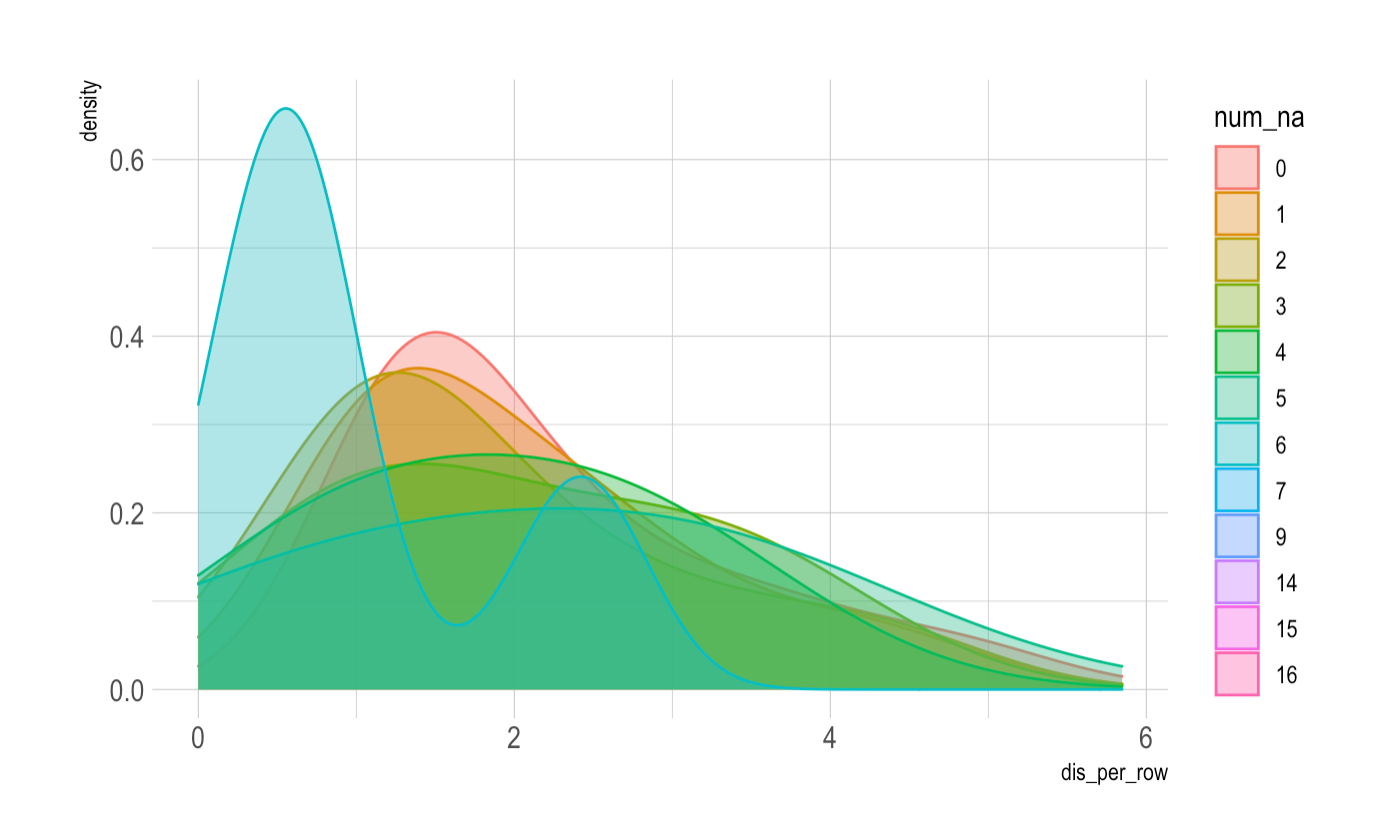
\includegraphics{https://github.com/wenxi77/PartialKmeans/blob/master/man/figures/housevotes_density.png}

}

\caption{Visualize the influence of the number of missing values for
each observation by drawing density plots of the distance between the
centroid and each observation. All distances are categorized by the
number of NAs in each observation.}

\end{figure}



\end{document}
